\section{Grey Level Models}
We can model the appearence of an object by examining
the statistics of grey levels in regions around each
of the labelled model points in the training images.
As with the shape, the grey-level environment can be
modelled by a mean and a number of modes of allowed variation.

For every landmark point $j$ in the image $i$ of the
training set, we extract a gray level profile $g_{ij}$ , of length
$np$ pixels, centered around the landmark point.
To reduce the effect of global intensity changes, we do not use
the actual vector $g$ but use the normalized derivative instead.

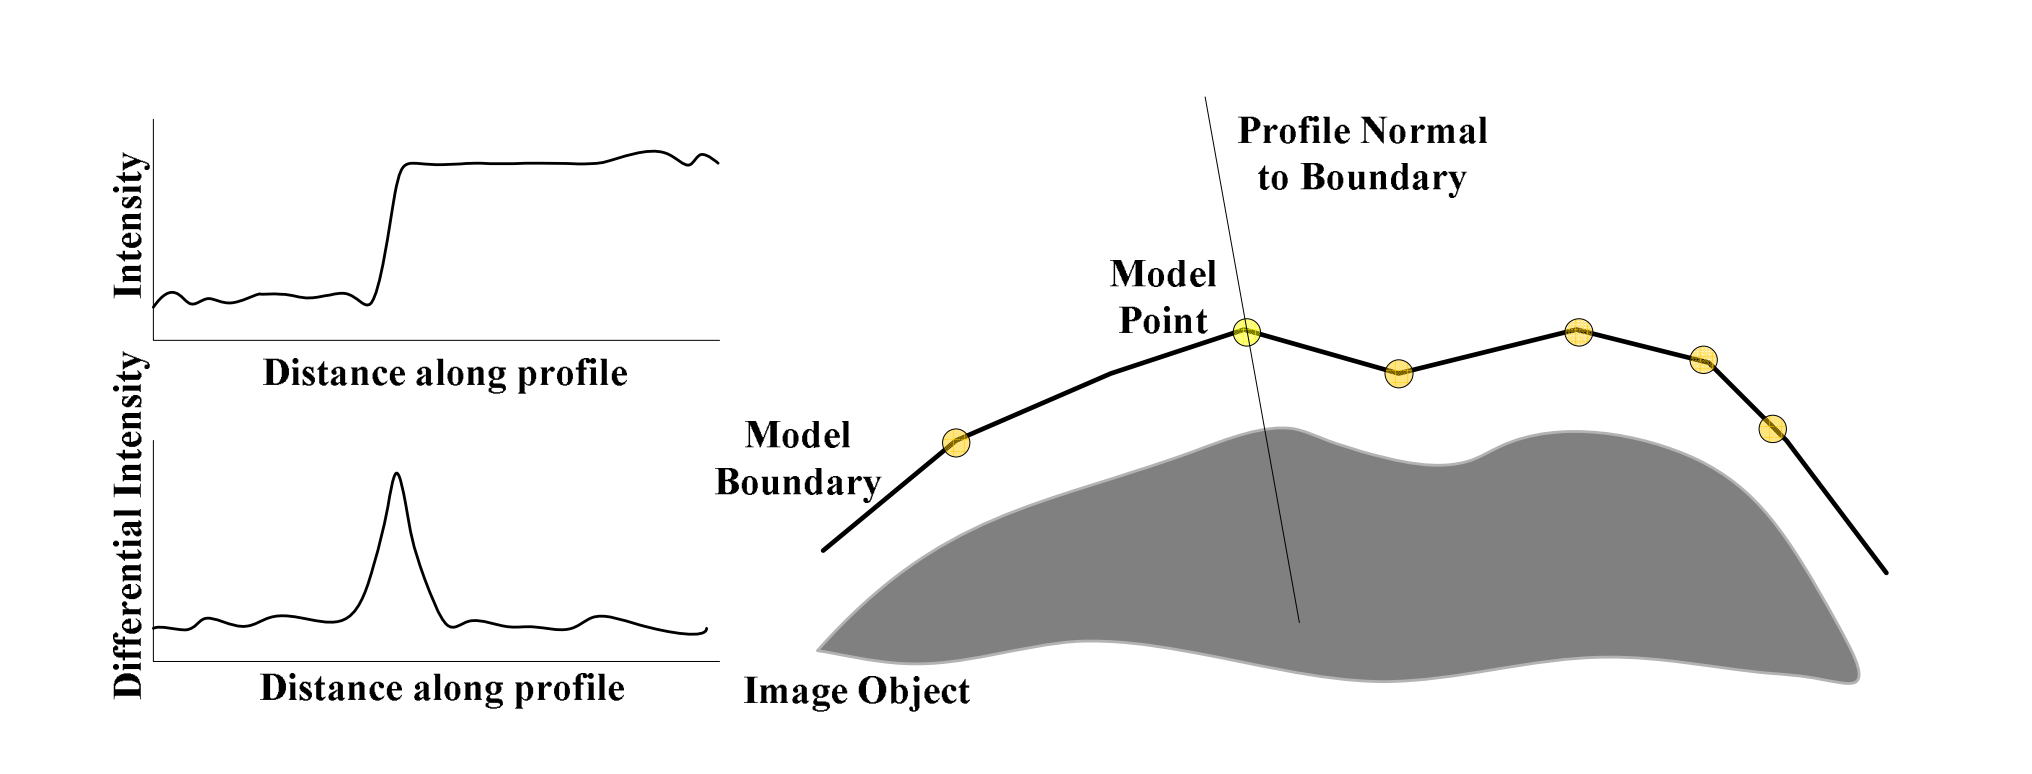
\includegraphics[width=\linewidth]{img/grey-level}